\documentclass[12pt]{article}

\usepackage{a4wide}
\usepackage[utf8]{inputenc}

\usepackage{graphicx}
\usepackage{palatino}
\usepackage{mathpazo}

%\pagestyle{empty}

\parindent=0pt
\begin{document}

\section*{Edge Thinning and Double Thresholding}

Today's exercise is focused on implementation of edge thinning and subsequent double thresholding to obtain clean edges.

\subsection*{Non-maxima Supression}

So far, we have used the Sobel operator or other convolution operators fo obtain edges in images.
These edges are rather thick.
Our goal is to get edges of image represend using a single pixel edges.
This is called edge thinning and we will use non-maxima supression to achieve this goal.
What non-maxima supression does is that it supresses (basically sets to 0) all values that are not maximum in ther context.
By context we mean the close neighbour of a pixel.
So in a 1D situation, we set leave unchanged on pixels that satisfy the following equation

\begin{equation} \label{eq:max_1d}
    E(x - 1) < E(x) > E(x + 1)
\end{equation}
As can be seen, retained value have to be bigger that the values on the left and right.
A simple illustration is depicted in Fig. \ref{fig:non-maxima-supression-1d}.

\begin{figure}[h]
\begin{centering}
    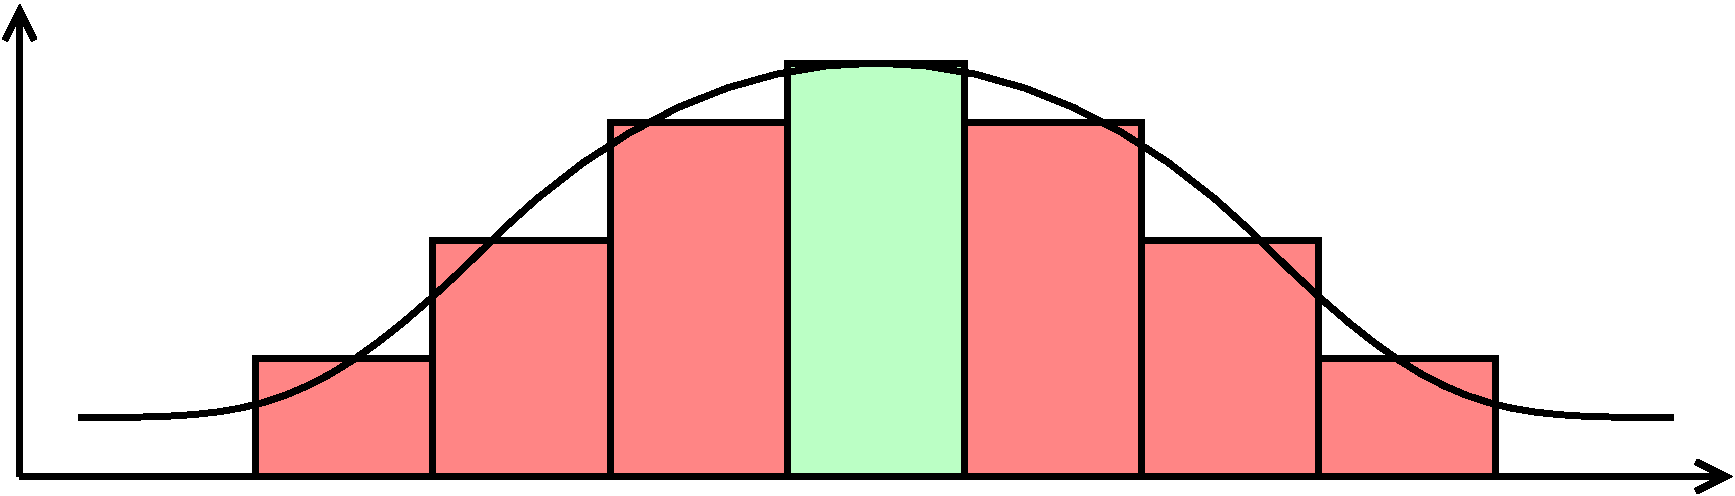
\includegraphics[width=0.6\textwidth]{non_maxima_supression_1d}
    \caption{An example of 1D non-maxima supression. Green and red bars represent function values at specific positions. The green value is retained, red values are non-maxima, so will be set to 0.}
    \label{fig:non-maxima-supression-1d}
\end{centering}
%\label{fig:non-maxima-supression-1d}
\end{figure}

\begin{figure}[h]
\begin{centering}
    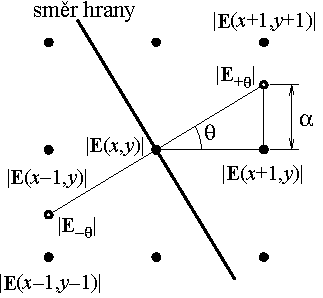
\includegraphics{pixel_scheme}
    \caption{An edge with corresponging gradient values (note that we use Cartesian coordinate system with the $(0, 0)$ coordinate in the bottom left, so adapt it later on in your code).}
    \label{fig:pixe-scheme}
\end{centering}
\end{figure}

\begin{equation}
    |E_{+\Theta}| = \alpha |E(x + 1, y + 1)| + (1 - \alpha) |E(x + 1, y)|
\end{equation}

\begin{equation}
    |E_{-\Theta}| = \alpha |E(x - 1, y - 1)| + (1 - \alpha) |E(x - 1, y)|
\end{equation}

\subsection*{Double Thresholding}

At this point, we have new image with edge magnitudes only at the centers of edges.
We have to separate real edges from random image pertubations.
To achieve this, we create two thresholds $t_1$ and $t_2$ that will be set by an experiment.
The only rule is to keep $t_2 > t_1$.

Double thresholding checks each edge magnitude $E(x, y)$ and if it is greater than $t2$ we set the pixel at coordinate $(x, y)$
in the output image to white (255). If the edge magnitude $E(x, y)$ is less than $t_2$ and but greater than $t_1$ and is
located next to the coordinate that has been already set as an edge, we set this coordinate as edge pixel too.

This algorithm may be easily implemented using recursive function. This function checks each edge magnitude and if labels
the coordinate as edge, it recursively calls itself in coordinates of top, bottom, left, and right neighbouring pixels.

\end{document}

